% context: 9th-grade physics homework, review for the Unit 1 measurement quiz
% topic: significant figures, rounding, scientific notation, reading a ruler,
%        unit conversion, average speed
% structure: four pages, problems widely spaced for written work
\documentclass[12pt, twoside]{article}
\input{../preamble}
\usepackage{float}

\title{Physics}
\author{Chris Huson}
\date{September 2026}

\fancyhead[LE]{\thepage}
\fancyhead[RO]{\thepage \\ Nickname: \hspace{2.25cm} \,\\ \,}
\fancyhead[LO]{La Scuola d'Italia / Huson / Physics \\* 18 September 2026}

\begin{document}

\subsubsection*{1.3 Homework: Measurement quiz review}

\textbf{Reference (provided).} \quad
average speed $= \dfrac{\text{distance}}{\text{time}}$ \\[0.1cm]
1 in. = 2.54 cm \quad 1 m $\approx$ 3.28 ft \quad 1 ft = 12 in \quad 1 mi = 5280 ft
\quad 1 mi $\approx$ 1.61 km \\
1 km = 1000 m \quad 1 m = 100 cm \quad 1 cm = 10 mm \quad 1 kg = 1000 g
\quad 1 gal $\approx$ 3.785 L \\
1 h = 3600 s \quad 1 min = 60 s \quad 1 yr $\approx 3.156 \times 10^{7}$ s

\vspace{0.25cm}

\begin{enumerate}[itemsep=0.5cm]

\item Write down the number of significant digits in each measurement.
  \begin{multicols}{3}
    \begin{enumerate}[itemsep=0.4cm]
      \item 48.5 m
      \item 0.0078 m
      \item 9.58 s
      \item 250.0 g
      \item 0.01070 kg
      \item $1.602 \times 10^{-19}$ C
    \end{enumerate}
  \end{multicols} \vspace{0.5cm}

\item Round each value to three significant figures. Copy the calculator display
  followed by three dots, then round: $\sqrt{2} = 1.4142135\ldots \approx 1.41$
  \begin{multicols}{2}
    \raggedright
    \begin{enumerate}[itemsep=1.3cm]
      \item $\sqrt{7}$
      \item The Earth--Moon distance, 384{,}400~km
    \end{enumerate}
  \end{multicols} \vspace{1.2cm}

\item Write in scientific notation, rounded to three significant figures.
  \begin{multicols}{2}
    \raggedright
    \begin{enumerate}[itemsep=1.3cm]
      \item The speed of light, 299{,}792{,}458 m/s
      \item The wavelength of green light, 0.000000532 m
    \end{enumerate}
  \end{multicols} \vspace{1.2cm}

\item Write each value as an ordinary decimal number.
  \begin{multicols}{2}
    \raggedright
    \begin{enumerate}[itemsep=1.3cm]
      \item The radius of the Earth, $6.37 \times 10^{6}$ m
      \item A GPS signal delay, $6.7 \times 10^{-2}$ s
    \end{enumerate}
  \end{multicols}

\newpage

\item The bar below is measured with a centimeter ruler marked in millimeters.

\begin{center}
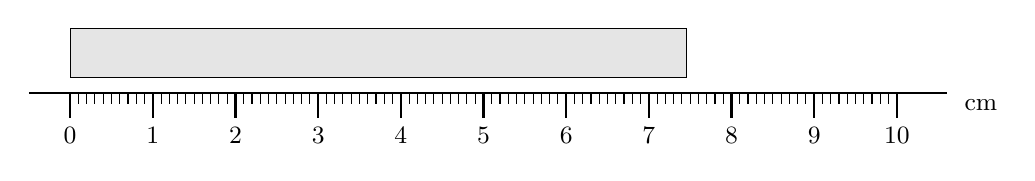
\begin{tikzpicture}[scale=1.05]
  \draw[fill=gray!20] (0,0.18) rectangle (7.45,0.78);
  \draw[thick] (-0.5,0) -- (10.6,0);
  \foreach \x in {0.1,0.2,...,9.95}{\draw (\x,0) -- (\x,-0.14);}
  \foreach \x in {0,1,2,3,4,5,6,7,8,9,10}{\draw[thick] (\x,0) -- (\x,-0.3) node[below] {\small \x};}
  \node[right] at (10.7,-0.15) {\small cm};
\end{tikzpicture}
\end{center}

  \begin{enumerate}[itemsep=0.9cm]
    \item Record the length of the bar. Include one estimated digit --- the last
      digit, the one you are not certain of.
    \item How many significant figures does your measurement have?
    \item Write the same length in millimeters, and again in meters.
  \end{enumerate} \vspace{1.0cm}

\item Convert between units. Write each conversion as a fraction and show the units
  cancelling.
  \begin{enumerate}[itemsep=2.6cm]
    \item One World Trade Center is 1776 feet tall. What is its height in meters?
    \item A US nickel has a mass of exactly 5.000 grams. What is the mass of a roll
      of 40 nickels, in kilograms?
  \end{enumerate} \vspace{2.4cm}

\item The marathon world record is 2 h 00 min 35 s for a distance of 42.195 km.
  Find the runner's average speed in meters per second, and again in kilometers per
  hour.

\newpage

\item A Frecciarossa train runs between Rome and Milan at 300 kilometers per hour.
  \begin{enumerate}[itemsep=2.6cm]
    \item What is this speed in meters per second?
    \item What is this speed in miles per hour?
  \end{enumerate} \vspace{2.4cm}

\item A badminton smash has been measured at 493 kilometers per hour --- the fastest
  projectile in any racket sport. A baseball fastball leaves the pitcher's hand at
  95 miles per hour.
  \begin{enumerate}[itemsep=2.4cm]
    \item Convert both speeds to meters per second.
    \item The pitcher's mound is 60.5 feet from home plate. How long does the
      fastball take to reach the plate? A typical human reaction time is 0.25 s ---
      what does your answer say about hitting a fastball?
  \end{enumerate} \vspace{2.2cm}

\item The mass of a proton is $1.673 \times 10^{-27}$ kg and the mass of an electron
  is $9.109 \times 10^{-31}$ kg. How many times more massive is the proton? Give your
  answer with the correct number of significant figures, and say why that is the
  right number.

\newpage

\item The Atlantic Ocean is widening at about 2.5 centimeters per year --- roughly
  the rate your fingernails grow.
  \begin{enumerate}[itemsep=2.8cm]
    \item Express this rate in meters per second, in scientific notation.
    \item How many years will it take the Atlantic to widen by 1.0 meter?
  \end{enumerate} \vspace{2.4cm}

\item A student measures the length of the hallway three times with a 30.0 m tape
  and records 24.1 m, 24.0 m, and 24.2 m.
  \begin{enumerate}[itemsep=1.5cm]
    \item What is the average of the three measurements?
    \item The student's calculator shows 24.1000000, and the student writes
      24.1000 m in the lab notebook. Explain what is wrong with that.
  \end{enumerate} \vspace{1.6cm}

\item Challenge: Gasoline in Rome costs \texteuro1.82 per liter. In New York it costs
  \$3.45 per gallon. On the day you check, \texteuro1 buys \$1.09.
  \begin{enumerate}[itemsep=1.6cm]
    \item What is the Rome price in dollars per gallon?
    \item How much more does a gallon cost in Rome than in New York?
    \item A Fiat's tank holds 45 liters. What does it cost, in dollars, to fill it
      in Rome?
  \end{enumerate}

\end{enumerate}
\end{document}
